\documentclass[notes,usenames,dvipsnames]{beamer}       % print frame + notes
% \documentclass[notes=only]{beamer}   % only notes
% \documentclass{beamer}              % only frames

% setting
\usepackage[labelformat=empty]{caption}
% \captionsetup{labelformat=empty}

\usepackage{xcolor}
\usepackage{minted}

\title{From Git to Heaven}
\subtitle{Go to heaven with your git commit}
\author{Azzam Syawqi Aziz}
% \date{}

% theme config
% \usetheme[
% outer/progressbar=foot,
% outer/numbering=none
% ]{metropolis}
\usetheme[outer/numbering=none]{metropolis}

% title case
\metroset{titleformat=smallcaps}

% title color
% \definecolor{Purple}{HTML}{3FFF00}
% \setbeamercolor{frametitle}{bg=Purple}

\begin{document}
\maketitle

\section{The Things}

\begin{frame}{I don't own those keys}
  \begin{figure}
    \centering
    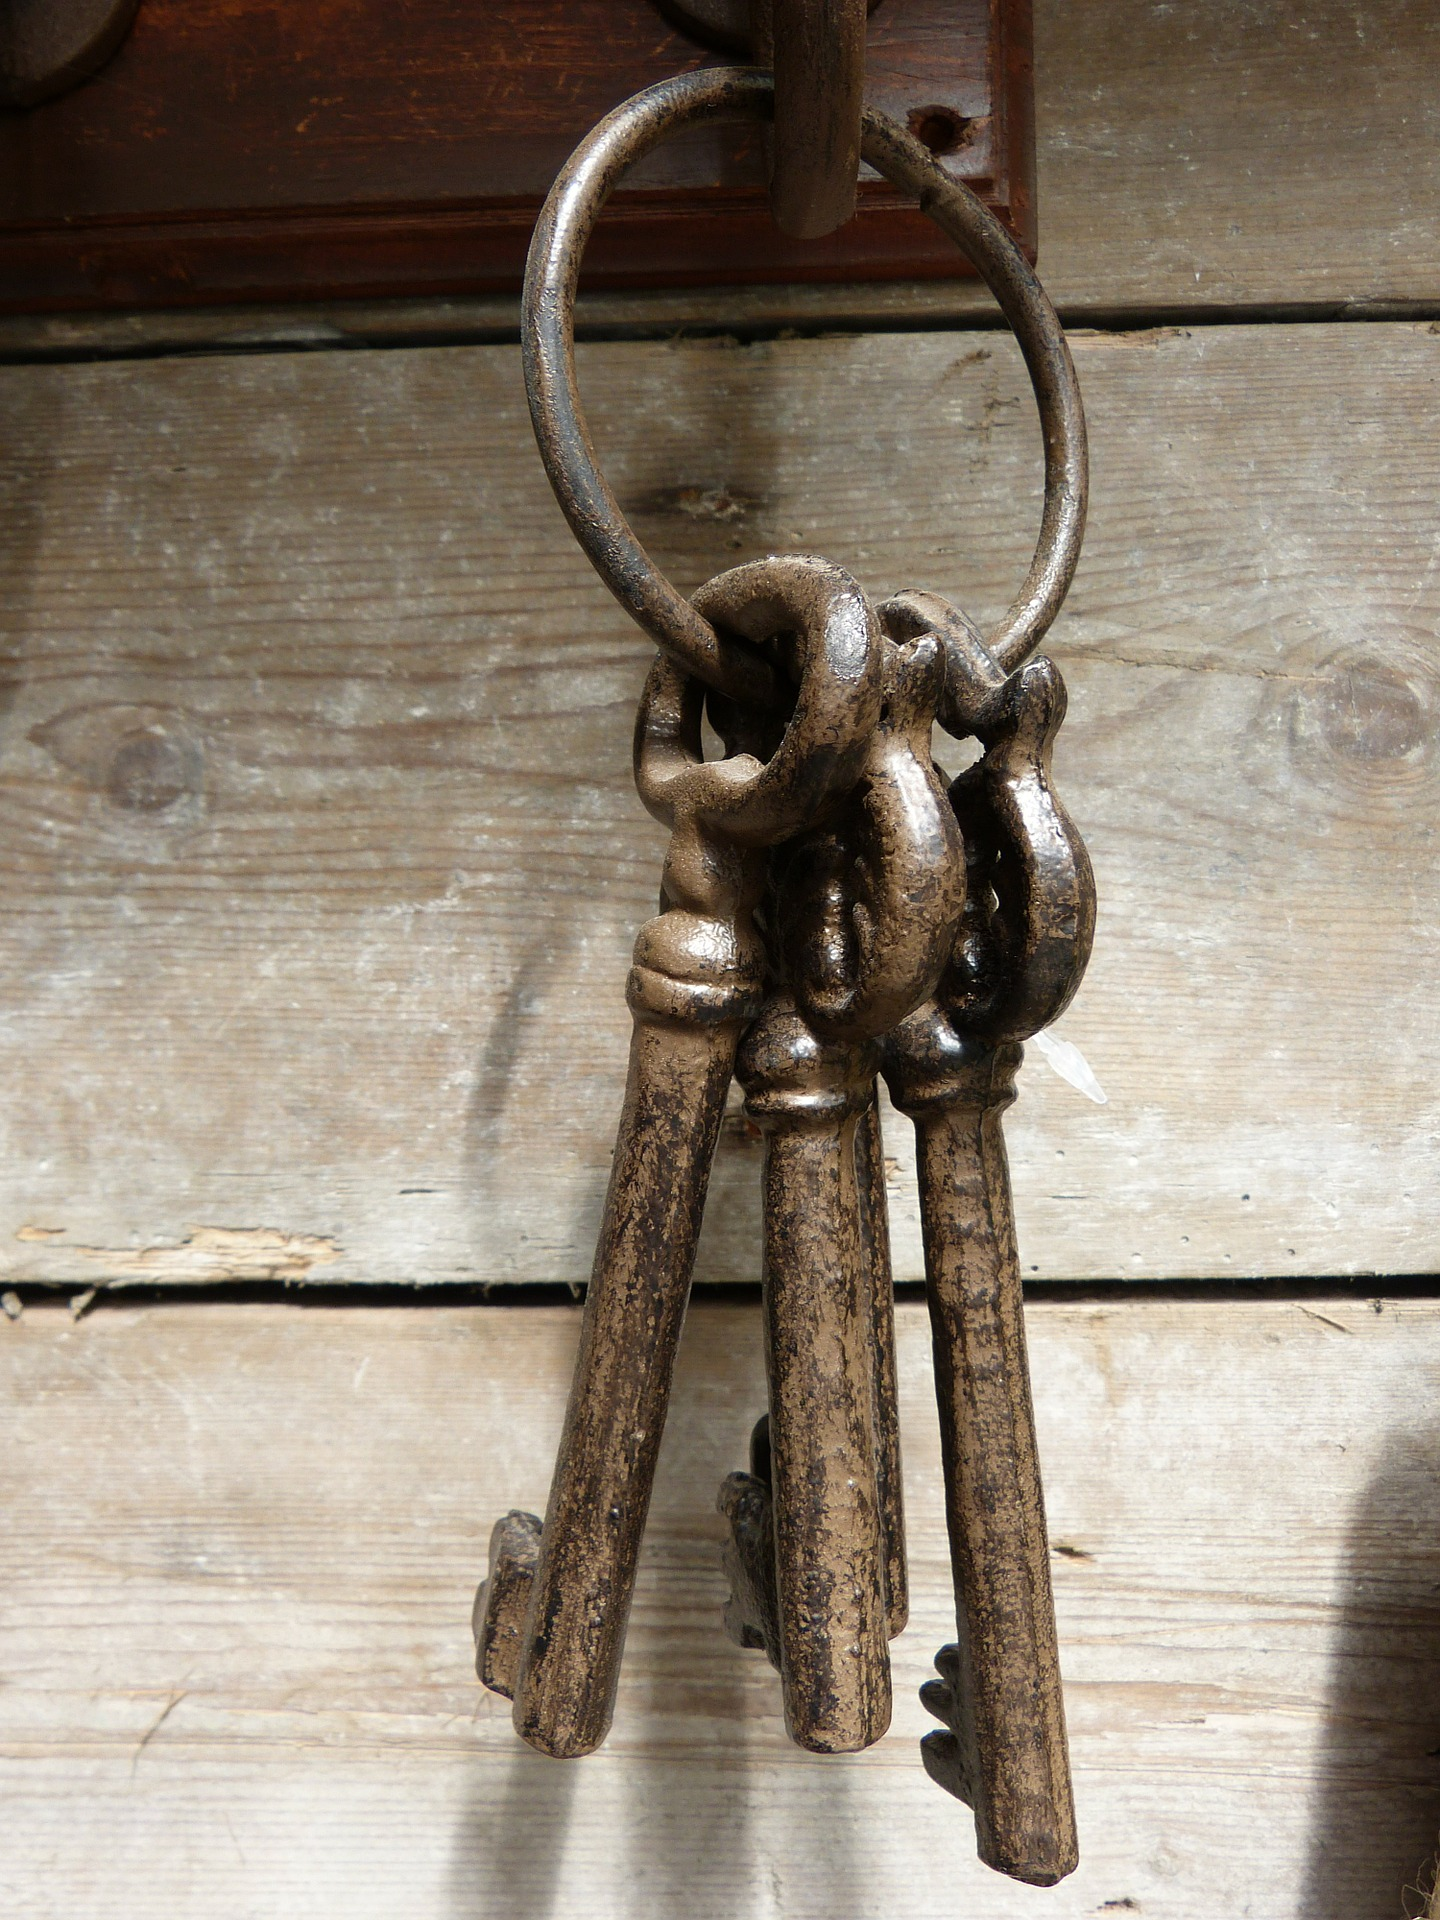
\includegraphics[scale=0.1]{img/key.jpg}
  \end{figure}
\end{frame}

\begin{frame}%{Small caps}
  \begin{center}
    \Huge SCM
  \end{center}
\end{frame}

\begin{frame}%{Small caps}
  \begin{center}
    \Huge Git
  \end{center}
\end{frame}

\begin{frame}%{Small caps}
  \begin{center}
    \Huge I don't use git anymore 😎
  \end{center}
\end{frame}

\section{The Concept}

\begin{frame}%{Small caps}
  \begin{center}
    \Huge Draw it!
  \end{center}
\end{frame}

\begin{frame}%{Small caps}
  \begin{center}
    \huge paste.debian.net/1023359/
  \end{center}
\end{frame}

% \begin{minted}[linenos,
% numbersep=5pt,
% gobble=2,
% frame=lines,
% framesep=2mm,
% fontsize=\tiny]{bash}
\begin{frame}[fragile]%{Small caps}
\begin{minted}[linenos,
frame=lines,
framesep=2mm,
fontsize=\tiny]{bash}
git init # create repo
git config --global user.name "name"
git config --global user.email "email"

git status
git add # move to staging area
git commit /-m # add to repo
git log # (sha-1)

# create new donuts!
git diff # diff wt <=> sa
git add */.
git diff --staged # diff sa <=> repo
git log -p
git rm
git checkout -- foo # restore from sa
git reset HEAD foo # restore from repo
\end{minted}
\end{frame}

\section{Branching and Merging}

\begin{frame}%{Small caps}
  \begin{center}
    \Huge Draw it!
  \end{center}
\end{frame}

\begin{frame}[fragile]%{Small caps}
\begin{minted}[linenos,
frame=lines,
framesep=2mm,
fontsize=\tiny]{bash}
git log --all --decorate --oneline --graph
git branch donat_pasir # (+ donat_besi)
git chekcout <branch>
# type of merge
git diff master..branch
git merge <baranch> # mostly HEAD->master
git branch --merged
git branch -d <branch>
git checkout -b # wohoo!
# make a bomb!
# detach -> gitk (or make branch)
git stash # save changes
git stash list/apply/pop
\end{minted}
\end{frame}

\section{Collaborate}

\begin{frame}%{Small caps}
  \begin{center}
    \Huge Draw it!
  \end{center}
\end{frame}

\begin{frame}[fragile]%{Small caps}
\begin{minted}[linenos,
frame=lines,
framesep=2mm,
fontsize=\tiny]{bash}
git clone
git remote add/remove
git fetch
git pull
git push
\end{minted}
\end{frame}

\section{Misc}

\begin{frame}{Tips}
  \begin{center}
    \begin{itemize}
    \item https://github.com/sindresorhus/refined-github
    \item https://github.com/magit/magit
    \end{itemize}
  \end{center}
\end{frame}

\begin{frame}{Futher Reading \& Credits}
  \begin{center}
    \begin{itemize}
    \item https://git-scm.com/docs/git-branch
    \item https://try.github.io/
    \item http://rogerdudler.github.io/git-guide/
    \item https://git-scm.com/book/en/v2
    \item  David Mahler Git video series
    \item https://marklodato.github.io/visual-git-guide/index-en.html
    \end{itemize}
  \end{center}
\end{frame}


\begin{frame}[standout]
  \Huge Questions?
\end{frame}


\end{document}
